
\documentclass[10pt]{article}
\usepackage{amsfonts,amsthm,amsmath,amssymb}
\usepackage{array}
\usepackage{epsfig}
\usepackage{fullpage}

%%% YOUR NAMES GO HERE %%%
\newcommand{\scribes}{Vahid Fazel-Rezai, Daniel Richman, Connor Sell}
%%% LECTURE NUMBER %%%
\newcommand{\lecnumber}{11}
%%% TITLE OF THE LECTURE %%%
\newcommand{\lectitle}{Semantically Secure Public-Key Encryption I
}
%%% DATE OF THE LECTURE %%%
\newcommand{\thedate}{Mar 9, 2016}

\begin{document}
%% Courtesy: Daniel Spielman, via Madhu Sudan --> Vinod Vaikuntanathan --> Aloni Cohen

%--------------
%% preamble.tex
%% this should be included with a command like
%% \input{preamble.tex}
%% \lecture{1}{September 4, 1996 }{Daniel A. Spielman}{name
%%  of poor scribe}


\hbadness=10000
\vbadness=10000

\newcommand{\handout}[6]{
   \renewcommand{\thepage}{#1 | Lec#6 | \arabic{page}}
   \noindent
   \begin{center}
   \framebox{
      \vbox{
    \hbox to 5.78in { {\bf #1}
     	 \hfill #2 }
       \vspace{4mm}
       \hbox to 5.78in { {\Large \hfill #5  \hfill} }
       \vspace{2mm}
       \hbox to 5.78in { {\it #3 \hfill #4} }
      }
   }
   \end{center}
   \vspace*{4mm}
}

\newcommand{\lecture}[4]{\handout{#1}{#2}{Lecturer:
#3}{Scribe: #4}{Lecture #1}}

\newtheorem{theorem}{Theorem}
\newtheorem{corollary}[theorem]{Corollary}
\newtheorem{lemma}[theorem]{Lemma}
\newtheorem{observation}[theorem]{Observation}
\newtheorem{proposition}[theorem]{Proposition}
\newtheorem{definition}[theorem]{Definition}
\newtheorem{claim}[theorem]{Claim}
\newtheorem{fact}[theorem]{Fact}
\newtheorem{assumption}[theorem]{Assumption}


%%%% GENERAL COMMANDS %%%%%%%%%%%%%%%%%%%%%%%%%%%%%%%%%


\newcommand{\dis}{\mathop{\mbox{\rm d}}\nolimits}
\newcommand{\per}{\mathop{\mbox{\rm per}}\nolimits}
\newcommand{\area}{\mathop{\mbox{\rm area}}\nolimits}
\newcommand{\cw}{\mathop{\rm cw}\nolimits}
\newcommand{\ccw}{\mathop{\rm ccw}\nolimits}
\newcommand{\DIST}{\mathop{\mbox{\rm DIST}}\nolimits}
\newcommand{\OP}{\mathop{\mbox{\it OP}}\nolimits}
\newcommand{\OPprime}{\mathop{\mbox{\it OP}^{\,\prime}}\nolimits}
\newcommand{\ihat}{\hat{\imath}}
\newcommand{\jhat}{\hat{\jmath}}
\newcommand{\abs}[1]{\mathify{\left| #1 \right|}}


%%%%% PROOF ENVIRONMENTS %%%%%%%%%%%%%%%%%%%%%%%%%%%%%%%%%%%%%%%%%%%%%%%%%%%%%%%%%%%%

\newenvironment{proof-sketch}{\noindent{\bf Sketch of Proof}\hspace*{1em}}{\qed\bigskip}
\newenvironment{proof-idea}{\noindent{\bf Proof Idea}\hspace*{1em}}{\qed\bigskip}
\newenvironment{proof-of-lemma}[1]{\noindent{\bf Proof of Lemma #1}\hspace*{1em}}{\qed\bigskip}
\newenvironment{proof-attempt}{\noindent{\bf Proof Attempt}\hspace*{1em}}{\qed\bigskip}
\newenvironment{proofof}[1]{\noindent{\bf Proof}
of #1:\hspace*{1em}}{\qed\bigskip}
\newenvironment{remark}{\noindent{\bf Remark}\hspace*{1em}}{\bigskip}

% \makeatletter
% \@addtoreset{figure}{section}
% \@addtoreset{table}{section}
% \@addtoreset{equation}{section}
% \makeatother

\newcommand{\FOR}{{\bf for}}
\newcommand{\TO}{{\bf to}}
\newcommand{\DO}{{\bf do}}
\newcommand{\WHILE}{{\bf while}}
\newcommand{\AND}{{\bf and}}
\newcommand{\IF}{{\bf if}}
\newcommand{\THEN}{{\bf then}}
\newcommand{\ELSE}{{\bf else}}

% \renewcommand{\thefigure}{\thesection.\arabic{figure}}
% \renewcommand{\thetable}{\thesection.\arabic{table}}
% \renewcommand{\theequation}{\thesection.\arabic{equation}}

\makeatletter
\def\fnum@figure{{\bf Figure \thefigure}}
\def\fnum@table{{\bf Table \thetable}}
\long\def\@mycaption#1[#2]#3{\addcontentsline{\csname
  ext@#1\endcsname}{#1}{\protect\numberline{\csname
  the#1\endcsname}{\ignorespaces #2}}\par
  \begingroup
    \@parboxrestore
    \small
    \@makecaption{\csname fnum@#1\endcsname}{\ignorespaces #3}\par
  \endgroup}
\def\mycaption{\refstepcounter\@captype \@dblarg{\@mycaption\@captype}}
\makeatother


\newcommand{\figcaption}[1]{\mycaption[]{#1}}
\newcommand{\tabcaption}[1]{\mycaption[]{#1}}
\newcommand{\head}[1]{\chapter[Lecture \##1]{}}
\newcommand{\mathify}[1]{\ifmmode{#1}\else\mbox{$#1$}\fi}
%\renewcommand{\Pr}[1]{\mathify{\mbox{Pr}\left[#1\right]}}
%\newcommand{\Exp}[1]{\mathify{\mbox{Exp}\left[#1\right]}}
\newcommand{\bigO}O
\newcommand{\set}[1]{\mathify{\left\{ #1 \right\}}}
\def\half{\frac{1}{2}}


% Command that ignores input.
\newcommand{\remove}[1]{}
\newcommand{\ignore}[1]{}
\newenvironment{ignoreme}{\ignore{}{}}

%%%%%%%%%%%%%% LATTICES %%%%%%%%%%%%%%%%%%%%%%%%%%%%%%%%%%%%%%%%%%%%%%%%%%%%%%%%%


\def\hh{\sigma^{\text{\rm\tiny top}}}
\def\ph{\sigma^{\text{\rm\tiny bot}}}
\def\hM{M^{\text{\rm\tiny top}}}
\def\pM{M^{\text{\rm\tiny bot}}}
\def\lsb{\mathsf{lsb}}

\newcommand{\gapSVP}{\mathsf{gapSVP}}
\newcommand{\SIVP}{\mathsf{SIVP}}

\def\dlwe{\mathsf{DLWE}}


\def\Zp{\Z_p}
\newcommand{\ip}[1]{\langle #1 \rangle}
\def\Psibar{\overline{\Psi}}

%Security Parameter
\newcommand{\secparam}{\kappa}
\newcommand{\secp}{\secparam}

\newcommand{\svp}{\mathsf{SVP}}

% Vectors, Matrices and such

\def\veca{\vc{a}}
\def\vecb{\vc{b}}
\def\vecc{\vc{c}}
\def\vecd{\vc{d}}
\def\vece{\vc{e}}
\def\vecm{\vc{m}}
\def\vecs{\vc{s}}
\def\vect{\vc{t}}
\def\vecv{\vc{v}}
\def\vecx{\vc{x}}
\def\vecy{\vc{y}}

\def\Z{\mathbb{Z}}
\def\R{\mathbb{R}}
\def\Q{\mathbb{Q}}

% Changing QED symbol in claim proofs
\newenvironment{claimproof}{\begin{proof}
\renewcommand{\qedsymbol}{{$\blacksquare$}}
}{\end{proof}}

% Calligraphic and blackboard type letters.

\def\cA{{\cal A}}
\def\cB{{\cal B}}
\def\cC{{\cal C}}
\def\cD{{\cal D}}
\def\cE{{\cal E}}
\def\cF{{\cal F}}
\def\cG{{\cal G}}
\def\cH{{\cal H}}
\def\cI{{\cal I}}
\def\cJ{{\cal J}}
\def\cK{{\cal K}}
\def\cL{{\cal L}}
\def\cM{{\cal M}}
\def\cN{{\cal N}}
\def\cO{{\cal O}}
\def\cP{{\cal P}}
\def\cQ{{\cal Q}}
\def\cR{{\cal R}}
\def\cS{{\cal S}}
\def\cT{{\cal T}}
\def\cU{{\cal U}}
\def\cV{{\cal V}}
\def\cW{{\cal W}}
\def\cX{{\cal X}}
\def\cY{{\cal Y}}
\def\cZ{{\cal Z}}
%%%%%%%%%%%%%%%%%
\def\bbC{{\mathbb C}}
\def\bbE{{\mathbb E}}
\def\bbF{{\mathbb F}}
\def\bbG{{\mathbb G}}
\def\bbM{{\mathbb M}}
\def\bbN{{\mathbb N}}
\def\bbQ{{\mathbb Q}}
\def\bbR{{\mathbb R}}
\def\bbV{{\mathbb V}}
\def\bbZ{{\mathbb Z}}

\def\Zq{\bbZ_q}

%%%%%%%%%%%%%%%%%


% Rounding commands

\newcommand{\ceil}[1]{\left\lceil #1 \right\rceil}
\newcommand{\floor}[1]{\left\lfloor #1 \right\rfloor}
\newcommand{\round}[1]{\left\lfloor #1 \right\rceil}


% Other short-hands

\def\binset{\{0,1\}}
\def\pmset{\{\pm 1\}}
\def\ind{\mathbbm{1}}
%\def\ind{\mathbf{1}}

\newcommand{\norm}[1]{\left\| {#1} \right\|}
\newcommand{\norminf}[1]{\left\| {#1} \right\|_{\infty}}


% Assignments
\def\getsr{\stackrel{\scriptscriptstyle{\$}}{\gets}}
\def\getsd{{:=}}
%\def\bydef{\stackrel{.}{=}}
\def\bydef{\triangleq}
\def\getsf{{\gets}}



% Asymptotics

\def\poly{{\rm poly}}
\def\polylog{{\rm polylog}}
\def\polyloglog{{\rm polyloglog}}
\def\negl{{\rm negl}}
\newcommand{\ppt}{\mbox{{\sc ppt}}}
\def\Otilde{\widetilde{O}}

% Indistinguishability
\newcommand{\cind}{{\ \stackrel{c}{\approx}\ }}
\newcommand{\sind}{{\ \stackrel{s}{\approx}\ }}

% Complexity classes

\def\NP{\mathbf{NP}}
\def\Ppoly{{\mathbf{P}/\poly}}


% Cryptographic assumptions

\newcommand{\ddh}{\mathrm{DDH}}
\newcommand{\cdh}{\mathrm{CDH}}
\newcommand{\dlin}{\text{\rm $d$LIN}}
\newcommand{\lin}{\text{\rm Lin}}
\newcommand{\sxdh}{\mathrm{SXDH}}
\newcommand{\rsa}{\mathrm{RSA}}
\newcommand{\sis}{\mathrm{SIS}}
\newcommand{\isis}{\mathrm{ISIS}}
\newcommand{\lwe}{\mathsf{LWE}}
\newcommand{\qr}{\mathrm{QR}}


% Types of attacks

\newcommand{\adv}{\mathrm{Adv}}
\newcommand{\dst}{\mathrm{Dist}}
\newcommand{\leak}{\mathrm{Leak}}
\newcommand{\forge}{\mathrm{Forge}}
\newcommand{\col}{\mathrm{Col}}
\newcommand{\invt}{\mathrm{Inv}}
\newcommand{\cpa}{\text{\rm CPA}}
\newcommand{\kdm}{\mathrm{KDM}}
\newcommand{\kdi}{\mathrm{KDM}^{(1)}}
\newcommand{\kdmn}{\mathrm{KDM}^{(\usr)}}
\newcommand{\ibe}{\mathrm{IBE}}
\newcommand{\good}{\mathrm{GOOD}}
\newcommand{\legal}{\mathrm{L}}


% Quadratic residuosity related

\newcommand{\qrs}{\mathbb{QR}}
\newcommand{\js}{\mathbb{J}}


% Linear algebra

\newcommand{\mx}[1]{\mathbf{{#1}}}
\newcommand{\vc}[1]{\mathbf{{#1}}}
\newcommand{\gvc}[1]{\bm{{#1}}}
%\newcommand{\vc}[1]{\gvc{{#1}}}

\newcommand{\rk}{\text{\rm Rk}}
\newcommand{\spn}{\text{\rm Span}}

% Probability

\newcommand{\Ex}{\mathop{\bbE}}
\newcommand{\cov}{\mathop{\text{\rm Cov}}}

%\newcommand{\sd}{\mathop{\text{\tt dist}}}
\newcommand{\sd}{\mathop{\Delta}}


% Entropy

\newcommand{\mH}{\mathbf{H_{\infty}}}
\newcommand{\avgmH}{\mathbf{\widetilde{H}_{\infty}}}


% Cryptographic elements

\newcommand{\pk}{{pk}}
\newcommand{\evk}{{evk}}
\newcommand{\pp}{{pp}}
\newcommand{\sk}{{sk}}
\newcommand{\vk}{{vk}}
\newcommand{\td}{{td}}

\newcommand{\msk}{{msk}}
\newcommand{\id}{{id}}

\newcommand{\crs}{\text{\sf crs}}

\newcommand{\params}{{params}}
\newcommand{\state}{{setupstate}}

\newcommand{\query}{{query}}
\newcommand{\qstate}{{qstate}}
\newcommand{\resp}{{resp}}


% Algorithms


\newcommand{\keygen}{\mathsf{Keygen}}
\newcommand{\gen}{\mathsf{Gen}}
\newcommand{\eval}{\mathsf{Eval}}
\newcommand{\setup}{\mathsf{Setup}}
\newcommand{\extract}{\mathsf{Extract}}
\newcommand{\enc}{\mathsf{Enc}}
\newcommand{\dec}{\mathsf{Dec}}

\newcommand{\symname}{\mathsf{SYM}}
\newcommand{\symkeygen}{\mathsf{SYM.Keygen}}
\newcommand{\symgen}{\symkeygen}
\newcommand{\symenc}{\mathsf{SYM.Enc}}
\newcommand{\symdec}{\mathsf{SYM.Dec}}


\newcommand{\shname}{\mathsf{SH}}
\newcommand{\shkeygen}{\mathsf{SH.Keygen}}
\newcommand{\shgen}{\shkeygen}
\newcommand{\shenc}{\mathsf{SH.Enc}}
\newcommand{\shdec}{\mathsf{SH.Dec}}
\newcommand{\sheval}{\mathsf{SH.Eval}}

\newcommand{\hename}{\mathsf{HE}}
\newcommand{\hekeygen}{\mathsf{HE.Keygen}}
\newcommand{\hegen}{\hekeygen}
\newcommand{\heenc}{\mathsf{HE.Enc}}
\newcommand{\hedec}{\mathsf{HE.Dec}}
\newcommand{\heeval}{\mathsf{HE.Eval}}


\newcommand{\fhname}{\mathsf{FH}}
\newcommand{\fhkeygen}{\mathsf{FH.Keygen}}
\newcommand{\fhenc}{\mathsf{FH.Enc}}
\newcommand{\fhdec}{\mathsf{FH.Dec}}
\newcommand{\fheval}{\mathsf{FH.Eval}}

\newcommand{\btsname}{\mathsf{BTS}}
\newcommand{\btkeygen}{\mathsf{BTS.Keygen}}
\newcommand{\btgen}{\btkeygen}
\newcommand{\btenc}{\mathsf{BTS.Enc}}
\newcommand{\btdec}{\mathsf{BTS.Dec}}
\newcommand{\bteval}{\mathsf{BTS.Eval}}

\newcommand{\fhename}{\mathsf{FHE}}
\newcommand{\fhekeygen}{\mathsf{FHE.Keygen}}
\newcommand{\fhegen}{\fhekeygen}
\newcommand{\fheenc}{\mathsf{FHE.Enc}}
\newcommand{\fhedec}{\mathsf{FHE.Dec}}
\newcommand{\fheeval}{\mathsf{FHE.Eval}}



\newcommand{\kdmkeygen}{\mathsf{KDM.Keygen}}
\newcommand{\kdmenc}{\mathsf{KDM.Enc}}
\newcommand{\kdmdec}{\mathsf{KDM.Dec}}

\newcommand{\vssgen}{\mathsf{VSS.Gen}}

\newcommand{\pirname}{\mathsf{PIR}}
\newcommand{\pirsetup}{\mathsf{PIR.Setup}}
\newcommand{\pirquery}{\mathsf{PIR.Query}}
\newcommand{\piranswer}{\mathsf{PIR.Response}}
\newcommand{\pirresp}{\piranswer}
\newcommand{\pirdec}{\mathsf{PIR.Decode}}




% Document specific definitions

\newcommand{\idl}[1]{\left\langle{#1}\right\rangle}
\newcommand{\rlwe}{\mathsf{RLWE}}
\newcommand{\plwe}{\mathsf{PLWE}}
\newcommand{\drlwe}{\text{\rm G-RLWE}}
\newcommand{\sdrlwe}{\text{\rm RLWE}}
\newcommand{\vssm}{\text{\rm SVSS}}

\newcommand{\ekdm}{{\cE_{\kdm}}}
\newcommand{\usr}{{\nu}}

\newcommand{\add}{\mathsf{add}}
\newcommand{\mlt}{\mathsf{mult}}

\newcommand{\hc}{\hat{c}}

\newcommand{\otild}{{\widetilde{O}}}
\newcommand{\omtild}{{\widetilde{\Omega}}}

\newcommand{\linf}{{\ell_{\infty}}}

\newcommand{\gf}{{\text{GF}}}

\newcommand{\zset}[1]{\{0, \ldots, {#1}\}}


\newcommand{\fig}[4]{
        \begin{figure}
        \setlength{\epsfysize}{#2}
        \vspace{3mm}
        \centerline{\epsfbox{#4}}
        \caption{#3} \label{#1}
        \end{figure}
        }

\newcommand{\ord}{{\rm ord}}

\providecommand{\norm}[1]{\lVert #1 \rVert}
\newcommand{\embed}{{\rm Embed}}
\newcommand{\qembed}{\mbox{$q$-Embed}}
\newcommand{\lp}{{\rm LP}}


\handout{6.875J/18.425J Cryptography and Cryptanalysis}
{\thedate}
{Instructor: Shafi Goldwasser}
{Scribes: \scribes}
{Lecture \lecnumber: \lectitle}
{\lecnumber}

%%%% body goes in here %%%%

Today's lecture focused on implementing \textit{public-key encryption}, especially RSA, and \textit{bit-by-bit encryption}. We also discussed techniques for implementing \textit{homomorphic encryption}, which enables some computation to be performed on encrypted data. 

\section{RSA preprocessing}

RSA has many nice properties. For example, every bit of the input is a hard-core bit for the trapdoor function family. But last lecture we also observed some flaws in the plain vanilla RSA encryption scheme:
\begin{itemize}
  \item Revealed information: for example, the Jacobi symbol of the ciphertext is equal to the Jacobi symbol of the message
  \item Determinism: RSA does not involve randomness, so a given message $m$ always encrypts to the same ciphertext $c$. This makes RSA insecure against chosen-ciphertext attacks
\end{itemize}

How can we fix these flaws? One approach is to nondeterministically preprocess the message before encrypting it with RSA. One scheme is Optimal Asymmetric Encryption Padding (OAEP) [BR94]:

\begin{figure}['h']
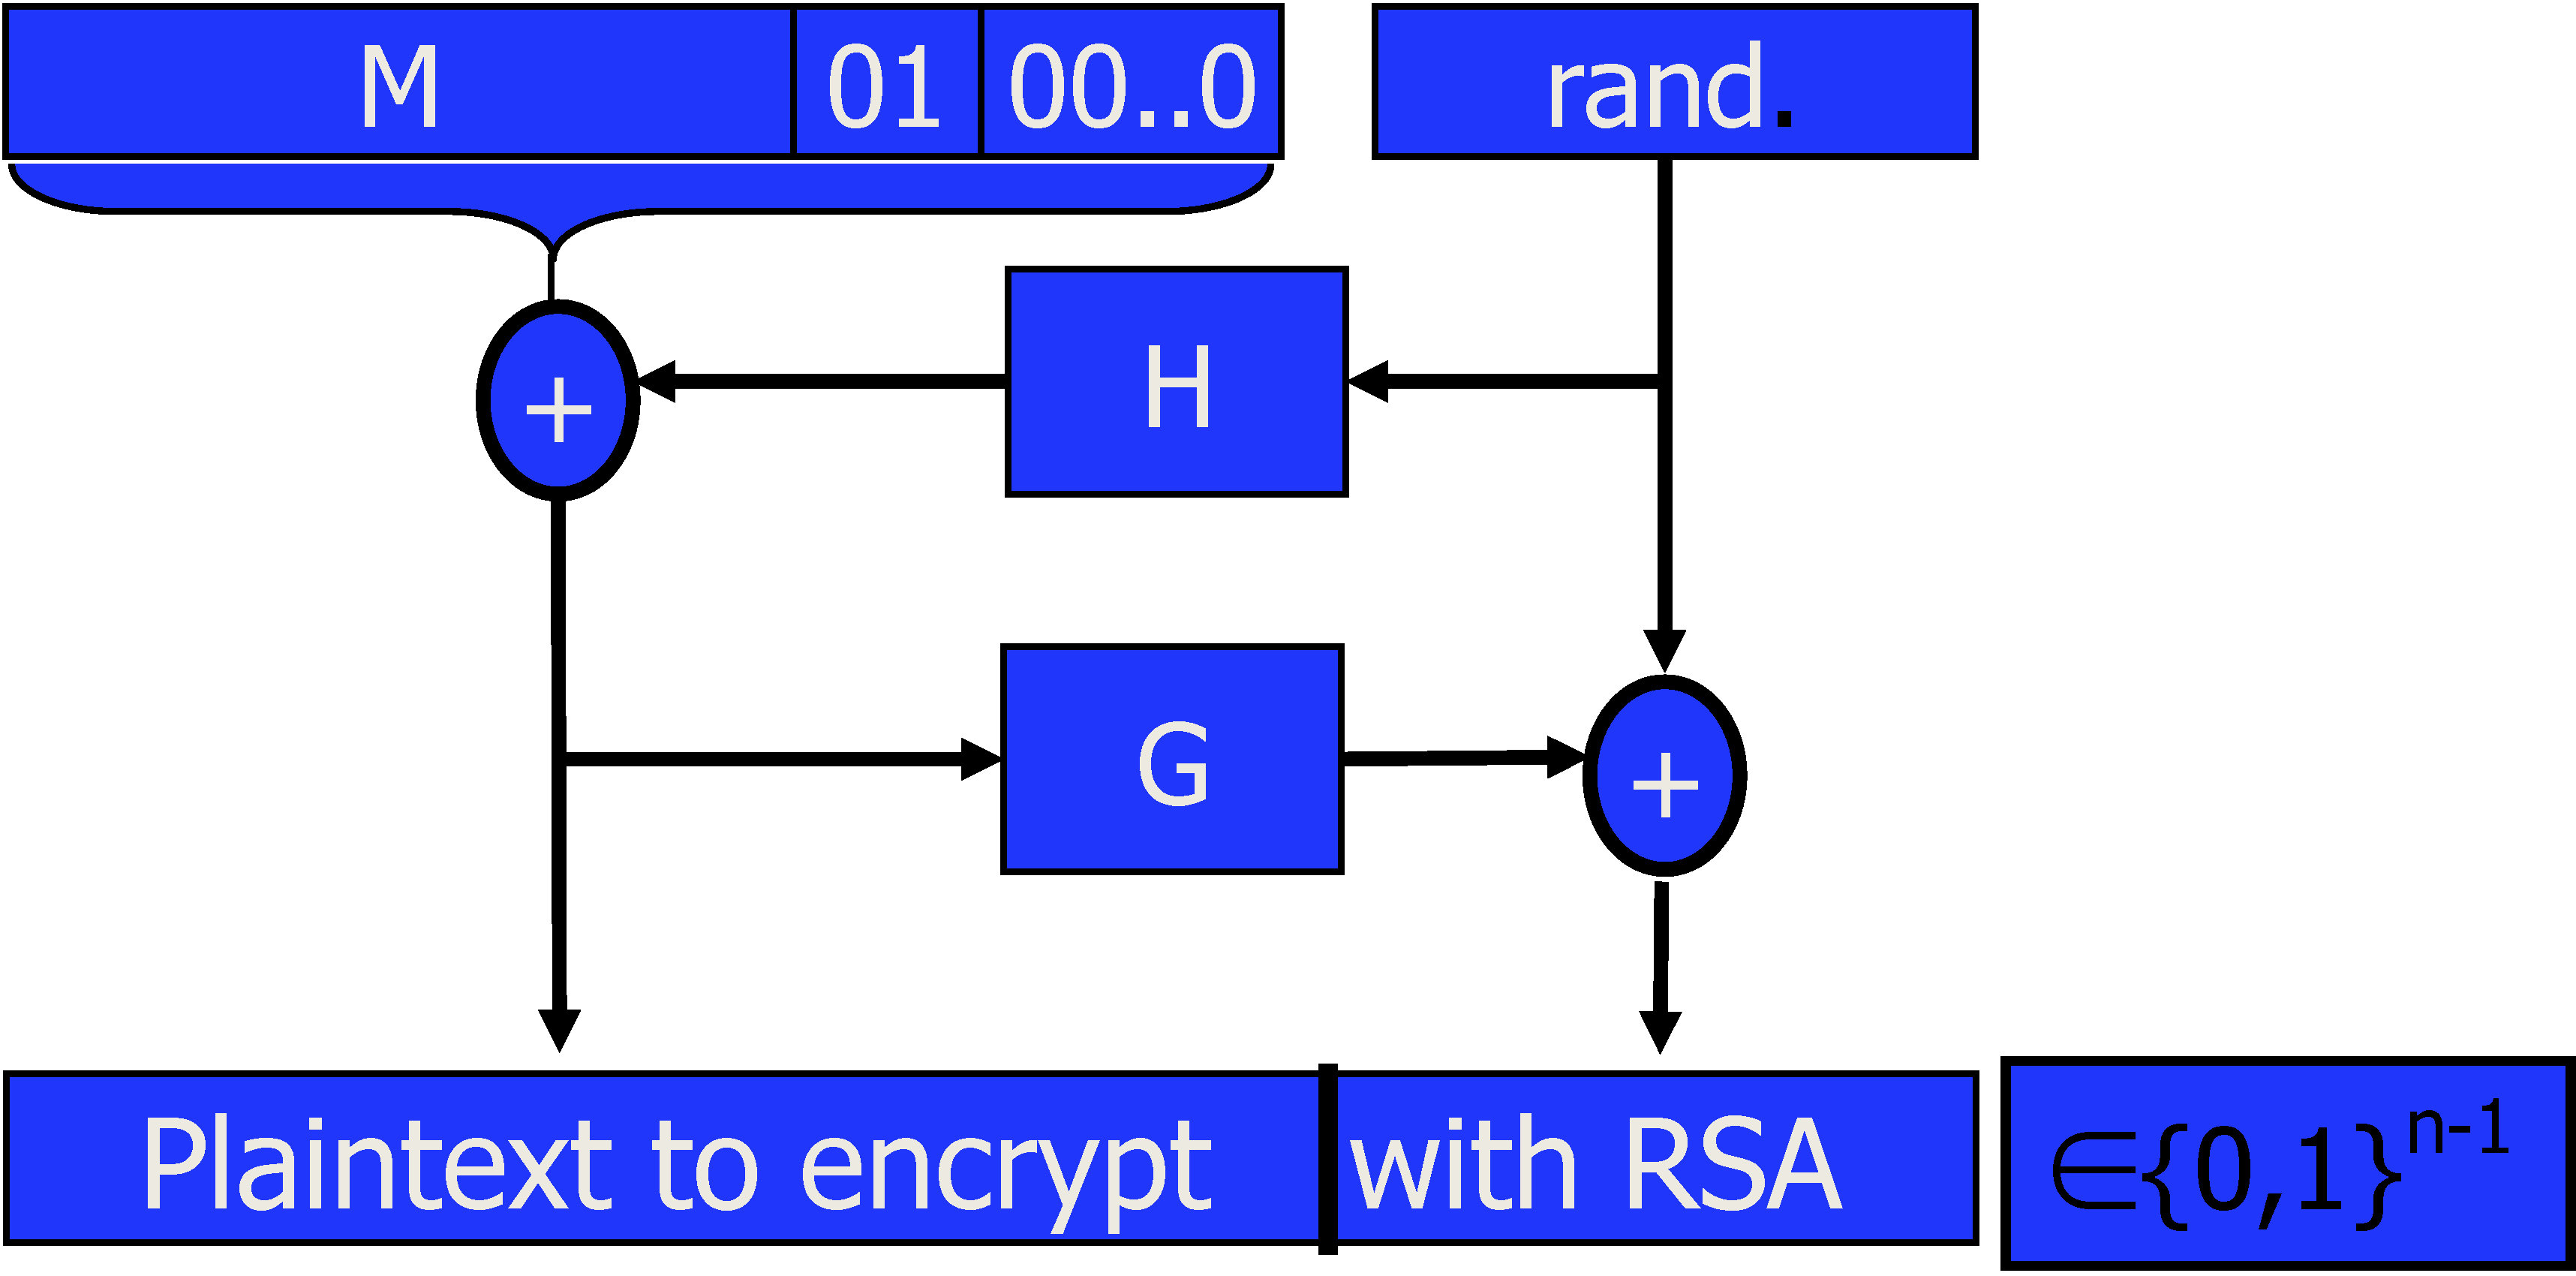
\includegraphics{oaep}
\caption{The OAEP block diagram}
\end{figure}

Theorem: OAEP is \textit{semantically secure} when H, G are \textit{random oracles}. Semantic security means that no partial information (other than the length of the message) is revealed by the ciphertext. The security holds under chosen-plaintext attacks and, when OAEP is used with RSA, under chosen-ciphertext attacks (CCA1) also. 

The padding bits $010\cdots 0$ make OAEP secure against 

\section{Random Oracles in Theory and Practice}

\section{Types of Attacks}

\begin{itemize}
	\item Lunchtime attack
	\item Timing attack
	\item Power attack
	\item Fault attack
	\item Cache attack
\end{itemize}

\section{Public key crypto based on squaring}

\section{Nondeterministic public key crypto with trapdoor functions}

\section{Trapdoor predicates}

\section{Using single-bit encryption for arbitrary length encryption}

\section{Homomorphic encryption and some primitives}

\section{Probabilistic encryption scheme and examples}





% % % You should probably leave the below alone % % %
\nocite{*}
\bibliographystyle{alpha}
\bibliography{scribe-bib}
\end{document}
